\documentclass{article}
\usepackage[utf8]{inputenc}

\usepackage{sectsty}
\usepackage{fancyhdr}
\usepackage[top=1.25cm, bottom=2cm, left=2cm, right=2cm]{geometry}
\usepackage{tabularx,tabulary}
\usepackage{graphicx}
\date{3 Avril 2019}
\author{FRANCESCHETTI Maël\\KADOCH Daoud\\MANSON Fabien\\CASTANET Nicolas}
\title{\LARGE{Projet 3i013\\}Rapport de Projet}

\usepackage[french]{babel}
%\usepackage[utf8x]{inputenc}
%\usepackage{amsmath}
%\usepackage[colorinlistoftodos]{todonotes}
\begin{document}

\begin{titlepage}

\newcommand{\HRule}{\rule{\linewidth}{0.5mm}} % Defines a new command for the horizontal lines, change thickness here

\center % Center everything on the page
 
%----------------------------------------------------------------------------------------
%	HEADING SECTIONS
%----------------------------------------------------------------------------------------

\textsc{\LARGE Université Pierre-et-Marie-Curie}\\[3cm] % Name of your university/college
\textsc{\Large Licence Informatique 3\up{ème} Année}\\[0.5cm] % Major heading such as course name
\textsc{\large Projet 3i013}\\[2cm] % Minor heading such as course title

%----------------------------------------------------------------------------------------
%	TITLE SECTION
%----------------------------------------------------------------------------------------

\HRule \\[0.4cm]
{ \huge \bfseries Rapport de Projet}\\[0.4cm] % Title of your document
\HRule \\[2cm]
 
%----------------------------------------------------------------------------------------
%	AUTHOR SECTION
%----------------------------------------------------------------------------------------

\begin{minipage}{0.4\textwidth}
	\begin{flushleft} \large
	\emph{Auteurs:}\\[0.2cm]
	Nicolas \textsc{CASTANET}\\ % Your name
	Maël \textsc{FRANCESCHETTI}\\ % Your name
	Daoud \textsc{KADOCH}\\ % Your name
	Fabien \textsc{MANSON} % Your name
	\end{flushleft}
\end{minipage}
~
\begin{minipage}{0.4\textwidth}
	\begin{flushright} \large
	\emph{Enseignant:} \\[0.2cm]
	Fabrice \textsc{KORDON}
	\end{flushright}
\end{minipage}\\[4cm]

%----------------------------------------------------------------------------------------
%	DATE SECTION
%----------------------------------------------------------------------------------------

{\large 3 Avril 2019}\\[3cm] % Date, change the \today to a set date if you want to be precise

%----------------------------------------------------------------------------------------
%	LOGO SECTION
%----------------------------------------------------------------------------------------


\includegraphics[scale=0.15]{logo_sorbonne.png} % Include a department/university logo - this will require the graphicx package
 
%----------------------------------------------------------------------------------------

\vfill % Fill the rest of the page with whitespace

\end{titlepage}

% -----------------------------------------------------
\newpage
\renewcommand{\contentsname}{\center{Table des Matières}\vspace*{5cm}}

\tableofcontents



\newpage
\section{Présentation du Projet}
	\subsection{Contexte}
		Un client nous souhaite effectuer un vol autonome avec un drone Bebop 2 tout en visualisant sur un iPod Touch le retour vidéo de la caméra embarquée sur le drone. L'iPod sera placé dans un masque de vue à la première personne. \\	
		%Le client souhaite faire effectuer des vols autonomes à un drone Bebop 2, avec un retour vidéo en temps réel sur un iPod Touch. Ce dernier pourra être placé dans un masque de vue à la première personne.\\
		La solution devra permettre à l'utilisateur de saisir un plan de vol sur une carte interactive et de le faire exécuter par le drone tout en ayant un retour vidéo sur l'iPod.\\
		
        

	\subsection{Solutions étudiées}
		%\vspace*{0.3cm}
		\begin{enumerate}
        	\item 
        	\item 
		\end{enumerate}
		
	\newpage
	\subsection{Use Case}	
	    \subsubsection{Création d'un plan de vol}
	    Dans le premier cas d'utilisation, l'utilisateur souhaite créer un nouveau plan de vol afin de le faire suivre à son drone dans le futur, voici les étapes qu'il va suivre:
	    
	    \vspace{0.7cm}	     
	    \begin{center}
	    \renewcommand{\arraystretch}{2}
        \begin{tabularx}{15cm}{|c|X|}
            \hline
            1 & L'utilisateur lance l'application et arrive sur la page d'accueil.\\
            \hline
            2 & L'utilisateur lance la fonctionnalité de saisie du plan de vol sur une machine connectée au réseau local.\\
            \hline
            3 & L'utilisateur saisit le plan de vol sur la carte en spécifiant les points de passage du drone ainsi que les altitudes que le drone doit adopter au cours du vol. \\
            \hline
            4 & L'utilisateur valide la saisie de son plan de vol, ce dernier est enregistré. \\
            \hline
        \end{tabularx}
        \end{center}
        
	    \vspace{0.8cm}
	    
	    \subsubsection{Excecution d'un plan de vol}
	    Dans le deuxième cas d'utilisaton, l'utilisateur possède déjà un ou plusieurs plan de vol enregistrés sur sa machine, par exemple le tour de son énorme jardin qu'il souhaite surveiller sans avoir à ce déplacer. Il fais désormais excécuter au drone l'un de ces plan de vol et observe le retour vidéo sur son Ipod.
	    Voici les étapes suivient :
	    
	    \vspace{0.7cm}	     
	    \begin{center}
	    \renewcommand{\arraystretch}{2}
        \begin{tabularx}{15cm}{|c|X|}
            \hline
            1 & L'utilisateur lance l'application et arrive sur la page d'accueil.\\
            \hline
            5 & L'utilisateur allume le drone et y connecte sa machine en wifi. \\
            \hline
            6 & L'utilisateur lance la fonctionnalité d'exécution du plan de vol. \\
            \hline
            7 &  L'utilisateur démarre l'iPod touch, le connecte au réseau local et lance l'application de réception vidéo. La réception vidéo en temps réel sur l'iPod commence.\\
            \hline
            8 & L'utilisateur sélectionne parmi les plans de vols présents sur le drone celui qu'il souhaite réaliser. \\
            \hline
            9 & L'utilisateur place l'iPod dans le masque FPV, le met sur sa tête, puis lance l'exécution du plan de vol. Le drone décolle. \\
            \hline
            10 & Le drone effectue le plan de vol choisi, l'utilisateur voit en temps réel ce que le drone filme et peut constater l'état d'enneigement de son jardin. \\
            \hline
            11 & L'utilisateur attend la fin de l'exécution du plan de vol pour retirer le masque et aller récupérer le drone une fois qu'il aura atterri à son point de départ, comme prévu.\\
            \hline 
\end{tabularx}
        \end{center}
	    
	    
	\newpage
	\subsection{Cahier des charges}

		
	\newpage
\section{Architecture Logicielle}
    \subsection{Interface utilisateur}
        \vspace*{0.5cm}
        \begin{center}
		\begin{figure}[!h]
		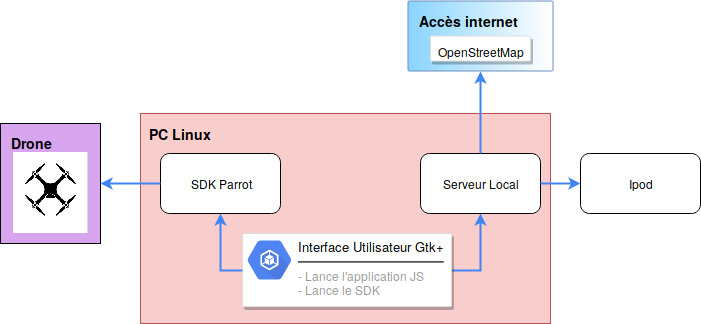
\includegraphics[scale=0.7]{Rapport/Interface_utilisateur.jpg}\\
		 \vspace*{0.3cm}
		\caption{Interface utilisateur}
		\end{figure}
        \end{center}

\newpage
        
	 \subsection{Controle du drone}
	    \vspace*{0.3cm}
	    \begin{center}
		\begin{figure}[!h]
		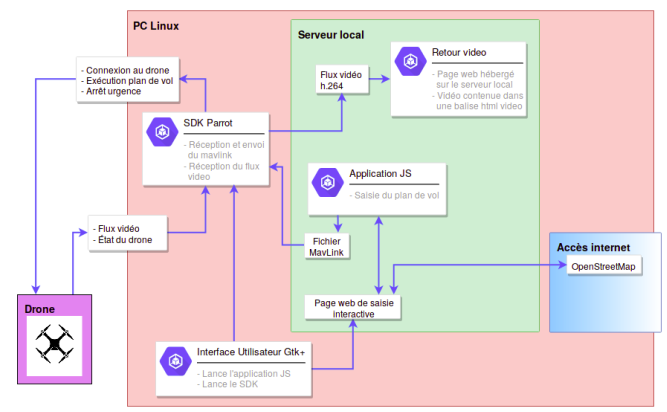
\includegraphics[scale=0.7]{Rapport/archi_controle_drone.png}\\
		\caption{Controle du drone}
		\end{figure}
        \end{center}
		
     \newpage
     \subsection{Application IOS}
        \vspace*{0.3cm}
	    \begin{center}
		\begin{figure}[!h]
		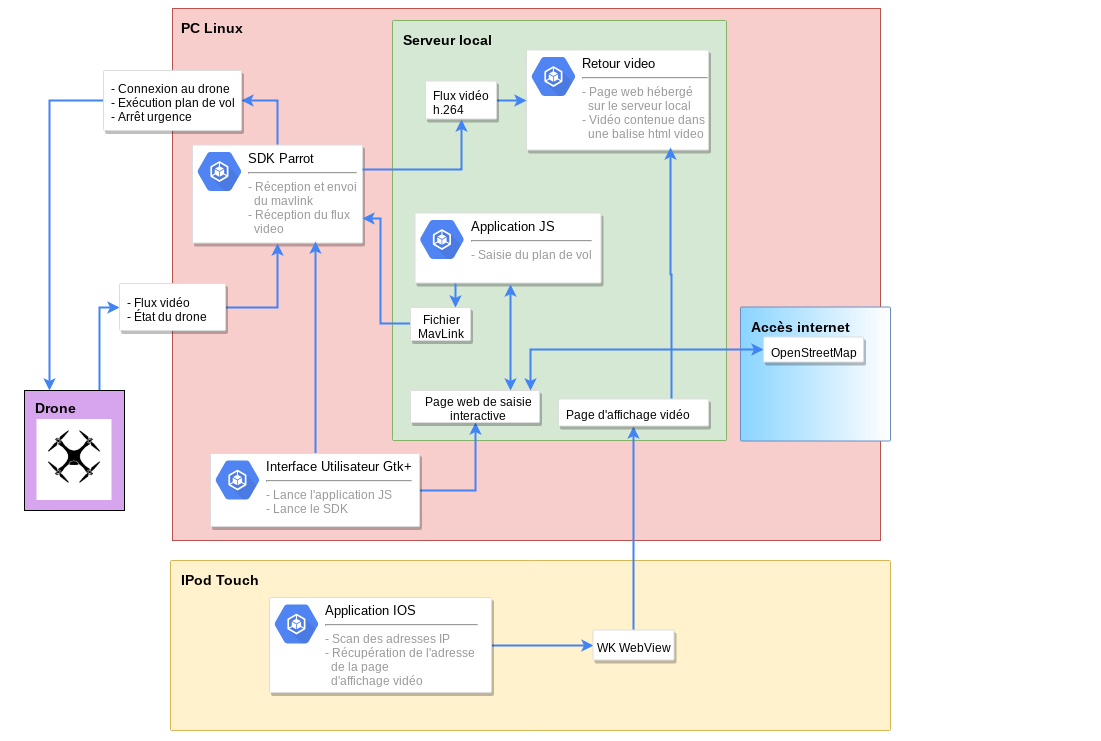
\includegraphics[scale=0.5]{Rapport/3_Architecture_logicielle_iPod.png}\\
		\caption{Application IOS}
		\end{figure}
        \end{center}
        
    \newpage
	
	\subsection{Architecture logicielle globale}
	    \vspace*{0.3cm}
	    \begin{center}
		\begin{figure}[!h]
		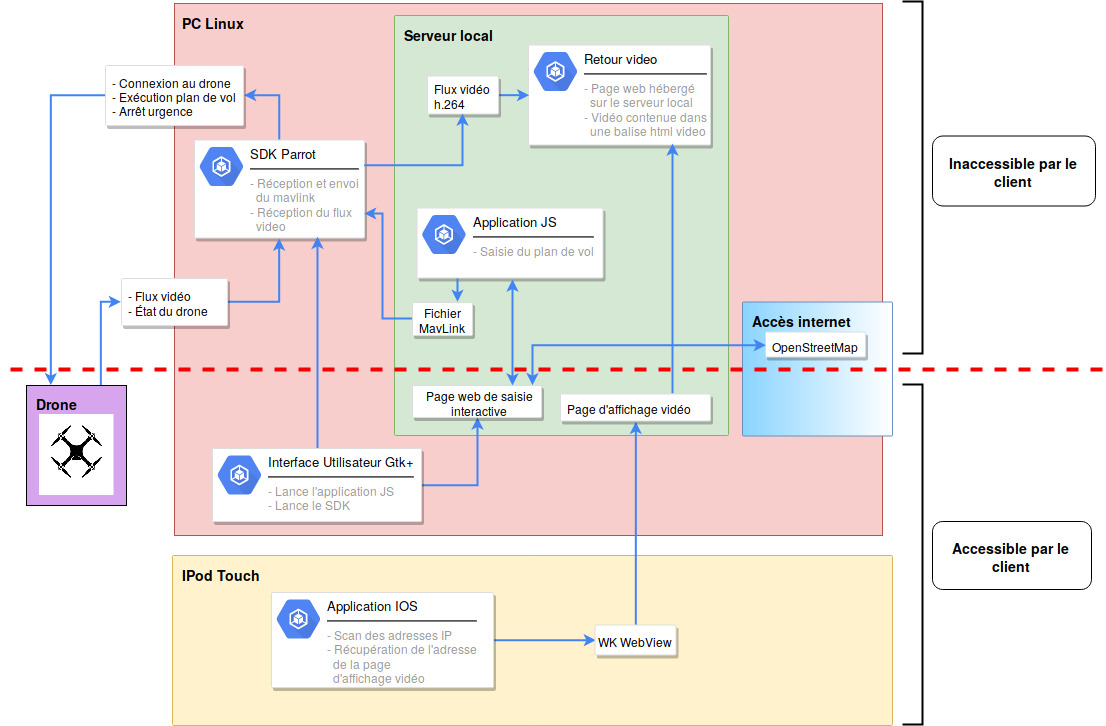
\includegraphics[scale=0.47]{Rapport/Architecture_logicielle_v2.jpg}\\
		\caption{Architecture logicielle}
		\end{figure}
        \end{center}
		
\newpage
\section{Problèmes rencontrés}
	\subsection{Problèmes matériels}
		
	
	\subsection{Solutions}
	
	

\newpage
\section{Organisation du travail}
	\subsection{Diagramme de Gantt}
        
	\subsection{Répartition des taches}
	
\section{Déploiement}


\newpage
\section{Comparatif aux objectifs fixés}
	
\newpage
\section{Améliorations possibles}


\newpage
\section{Conclusion}
	
 
\end{document}